\documentclass[12pt]{article}
\usepackage[a4paper, margin=2cm]{geometry}
\usepackage[english]{babel} % To obtain English text with the blindtext package
\usepackage{blindtext}
\usepackage{graphicx} % Required for inserting images
\usepackage{array} % For extra column formatting
\usepackage{amsmath, amssymb} %for equation environment
\usepackage{float}
\usepackage{parskip} % For gaps between para
\usepackage{setspace}
\usepackage{pdfpages}
\usepackage{abstract}
\usepackage[export]{adjustbox}
\usepackage{emptypage}
\usepackage{tocloft}
\usepackage[nottoc]{tocbibind}
\usepackage{hyperref, url}
\usepackage{subcaption}
\usepackage{lipsum}
\usepackage{xcolor}
\usepackage{caption}
    \captionsetup{font=footnotesize,labelfont=bf}

\cftsetindents{section}{0em}{2em}
\cftsetindents{subsection}{0em}{2em}

\renewcommand\cfttoctitlefont{\hfill\Large\bfseries}
\renewcommand\cftaftertoctitle{\hfill\mbox{}}

\graphicspath{ {./images/} }

\pagenumbering{arabic}

\definecolor{blurple}{HTML}{5865F2}

\hypersetup{
    colorlinks=true,
    linkcolor=black,
    urlcolor=blurple,
    citecolor=blurple,
}

\urlstyle{same}

\renewcommand{\arraystretch}{1.3}

%%%%%%%%%%%%%%%%%%%%%%%%%%%%%%%%%%%


\title{PHYC20080 Exp.1 Lenses}
\author{Joana Adao}
\date{\today}

\begin{document}

\begin{titlepage}
    \begin{center}

        \begin{figure}[ht]
            
\includegraphics[width=\textwidth]{UCDLogo.png}
        \end{figure}
        
        \begin{figure}
            \centerline{
\includegraphics[width=\paperwidth]{UCDBanner.png}}
        \end{figure}

        \vspace{4cm}

        {\LARGE \bfseries PHYC20080 Fields, Waves and Light}\\
        \vspace{0.75cm}
        {\Large Experiment No.1 Measurement of the Focal Lengths of Lenses and a Determination of Brewster's Angle}
        
        \vspace{1cm}
    
    {\Large \textbf{4 February 2025}}

    \vspace{2cm}
    
    {\large \textbf{by Joana C.C. Adao (Student No. 23311051)}}\\
    \vspace{0.25cm}
    {\large Tuesday 16.00-18.00 Slot}\\
    {\large Nicki (Coordinator)}

    \end{center}
    
   \clearpage

\end{titlepage}

\setcounter{page}{1}
\tableofcontents

\newpage

\begin{abstract}
\addcontentsline{toc}{section}{Abstract}

\vspace{1cm}

The aim of this experiment 

\end{abstract}

%%%%%%%%%%%%%%%%%%%%%%%%%%%%%%%%%%%

\section{Theory} \label{sec:1}

\subsection{Lenses} \label{sec:1.1}

Lenses are a piece of transparent materials, typically glass, that are used to bend and focus rays of light onto one spot to form images
\cite{britlens,vedantulens}.
Lenses can either be shaped to be concave (depressed, caved) or convex (bulging, rounded), but have to have at least one curved surface
\cite{britlens,vedantulens}
The properties that make up a lens are: \textit{focal length} (§\ref{sec:1.1.1}), \textit{focal point}, \textit{optical axis}, \textit{focus}, \textit{principal axis}, \textit{centre of curvature}
\cite{geekconcave,geekconvex}

\begin{figure}[H]
    \centering
    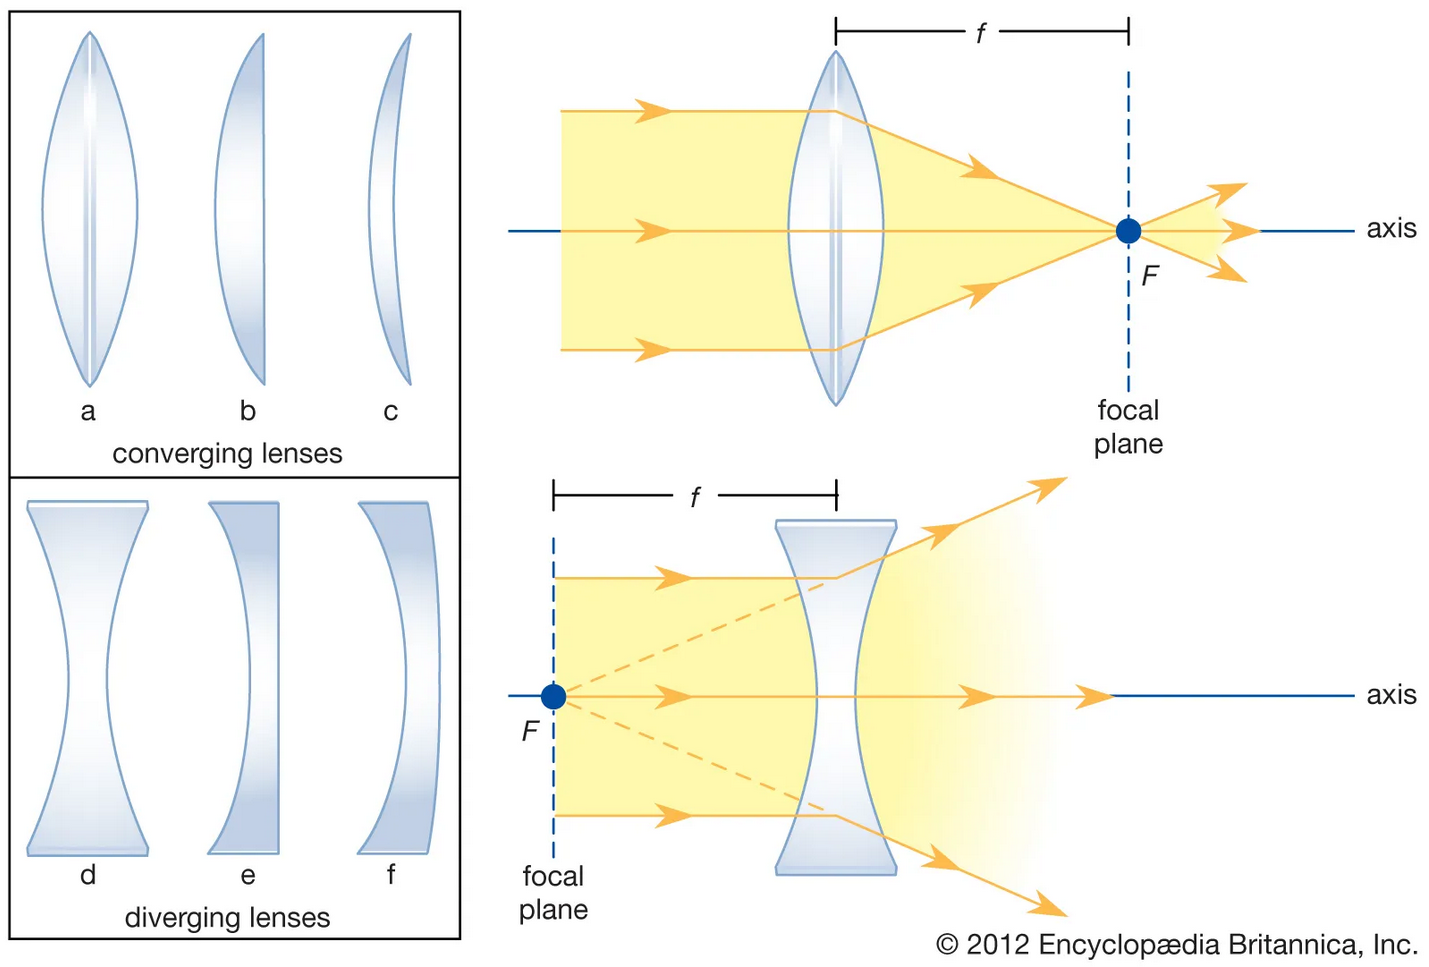
\includegraphics[width=15cm]{lenses.png}
    \caption{\centering Diagram of converging (convex) and diverging (concave) lenses \protect\cite{britlens}.
    \newline
    \centering \scriptsize{\textit{(a): biconvex, (b): plano-convex, (c): positive meniscus; (d): biconcave, (e): plano-concave, (f): negative meniscus}}}
    \label{fig:lens}
\end{figure}

Convex lenses make the parallel travelling rays of light passing through it \textbf{converge} to a certain point known as the \textit{focal point} (\ref{sec:1.1.1})
\cite{studyconvexlens}.
The degree at which light is bent depends on the absolute curvature of the lens
\cite{shanghaiconvex}.
The convex lens has two extra properties that do not apply to a concave lens: \textit{radius of curvature}, and \textit{aperture}
\cite{geekconvex}.
The behaviour of ligh as it passes through a convex lens can be simulated via the interactive diagram link in \textit{References}, §\ref{sec:ref}
\cite{convexinteract}.

Concave lenses make the parallel travelling rays of ligth passing through it \textbf{refract} away from the focal point of the lens
\cite{studyconvexlens,studyconcavelens}.
The behaviour of ligh as it passes through a concave lens can be simulated via the interactive diagram link in \textit{References}, §\ref{sec:ref}
\cite{concaveinteract}.

\subsubsection{Focal Length} \label{sec:1.1.1}

The focal length is the distance, typically in millimetres, of the \textit{optical axis} (the centre of the lens) to the focal plane shown in figure \ref{fig:lens}
\cite{canonfocal,studyfocal}.
The focal point, indicated by the point at which the focal plane and principal axis intersect, is the point at which the rays of light coincide
\cite{isaaclens}.
For a concave lens, where the light diverges, there only exists an \textit{apparent} focal point behind the lens, where a virtual image would be formed (§\ref{sec:1.1.2})
\cite{isaaclens}.

The formula below, equation \ref{eq:1}, is used to calculate the focal lenght of a thin converging lens \cite{UCDlens,isaaclens}, where \textbf{u} is the distance
between the \textit{object} and the centre of the lens, and \textbf{v} is the distance between the \textit{image} and the centre of the lens:

\begin{gather} \label{eq:1}
    \frac{1}{f} = \frac{1}{u} + \frac{1}{v}
\end{gather}

Since a concave lens does not form a real image (§\ref{sec:1.1.2}) one must add a convex lens to overcome this issue. Therefore equation \ref{eq:1} becomes invalid (individually) for calculating the focal length.
Instead, equation \ref{eq:2} below can be used to find the focal length of the combined lenses, where $f_{convex}$ (focal length of the convex lens) and $f_{concave}$ (focal length of the concave lens) can be calculated individually
using equation \ref{eq:1} \cite{UCDlens}:  

\begin{gather} \label{eq:2}
    \frac{1}{f} = \frac{1}{f_{convex}} + \frac{1}{f_{concave}}
\end{gather}

Concave lenses have \textit{negative} focal length, as opposed to convex lenses, since the focal point is on the same side as the incident (incoming) light \cite{geekconcave}.

\subsubsection{Image Formation} \label{sec:1.1.2}

Two types of images can be formed when looking at a mirror or through a lens:
\begin{itemize}
    \item \textbf{Real image:} an image formed when light converges at a point; inverted in nature \cite{geekrelvir}.
    \item \textbf{Virtual image:} an image formed when light diverges away from a point; appears to be produced but is not actually present \cite{geekrelvir}.
\end{itemize}

Standard image properties of convex lenses is that what is produced is a real image that is inverted and enlarged
\cite{geekconvex}, but virtual images can also be formed.
The image produced depends on the object position at the time of measurement.
The types of images convex lenses can form are illustrated in figure \ref{fig:conveximage} and described in table \ref{tab:1} (\textit{sourced directly from Geeksforgeeks \cite{geekconvex}}).

\begin{minipage}{.5\textwidth}
    \captionsetup{hypcap=false}
    \centering
    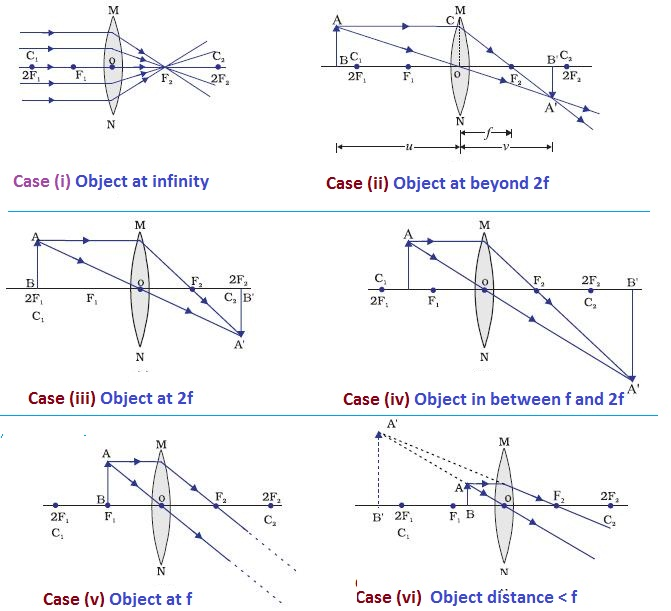
\includegraphics[width=.9\linewidth]{convex.jpg}
    \captionof{figure}{\centering Ray diagram of the cases of convex lens image formation \protect\cite{topprlensimage}.}
    \label{fig:conveximage}
\end{minipage}
\hfill
\begin{minipage}{.45\textwidth}
    \captionsetup{hypcap=false}
    \centering
    
    \begin{table}[H]
        \centering
        \resizebox{.9\linewidth}{!}{

            \begin{tabular}{|c|c|c|c|}
            \hline
            \textbf{\begin{tabular}[c]{@{}c@{}}Object\\ Position\end{tabular}}     & \textbf{\begin{tabular}[c]{@{}c@{}}Image\\ Position\end{tabular}} & \textbf{\begin{tabular}[c]{@{}c@{}}Image\\ Size\end{tabular}} & \textbf{\begin{tabular}[c]{@{}c@{}}Image\\ Nature\end{tabular}}                 \\ \hline
            \textbf{Beyond 2F}                                                     & \begin{tabular}[c]{@{}c@{}}Between \\ F and 2F\end{tabular}       & Smaller                                                       & \begin{tabular}[c]{@{}c@{}}Real,\\ Inverted\end{tabular}                        \\ \hline
            \textbf{At 2F}                                                         & At 2F                                                             & Same size                                                     & \begin{tabular}[c]{@{}c@{}}Real, \\ Inverted\end{tabular}                       \\ \hline
            \textbf{\begin{tabular}[c]{@{}c@{}}Between \\ F and 2F\end{tabular}}   & Beyond 2F                                                         & Larger                                                        & \begin{tabular}[c]{@{}c@{}}Real, \\ Inverted\end{tabular}                       \\ \hline
            \textbf{At F}                                                          & Infinity                                                          & Infinite                                                      & \begin{tabular}[c]{@{}c@{}}Real, \\ Inverted\\ (Highly Diminished)\end{tabular} \\ \hline
            \textbf{\begin{tabular}[c]{@{}c@{}}Between \\ F and lens\end{tabular}} & Beyond 2F                                                         & Larger                                                        & \begin{tabular}[c]{@{}c@{}}Virtual, \\ Upright\end{tabular}                     \\ \hline
            \textbf{At lens}                                                       & At lens                                                           & Larger                                                        & \begin{tabular}[c]{@{}c@{}}Virtual, \\ Upright\end{tabular}                     \\ \hline
            \textbf{\begin{tabular}[c]{@{}c@{}}Object inside \\ lens\end{tabular}} & \begin{tabular}[c]{@{}c@{}}Between \\ lens and F\end{tabular}     & Larger                                                        & \begin{tabular}[c]{@{}c@{}}Virtual, \\ Upright\end{tabular}                     \\ \hline
            \end{tabular}

        }
        \caption{\centering Table of the different cases of convex lens image formation \protect\cite{geekconvex,topprlensimage}.}
        \label{tab:1}
    \end{table}
\end{minipage}

Standard image properties of concave lenses is that what is produced is a virtual image that is upright and diminished
\cite{geekconcave}.
Concave lenses cannot produce real images. The only thing that changes between the virtual images that are produced is the magnitude at which they're diminished
\cite{topprlensimage,geekconcave}.

\begin{minipage}{.5\textwidth}
    \captionsetup{hypcap=false}
    \centering
    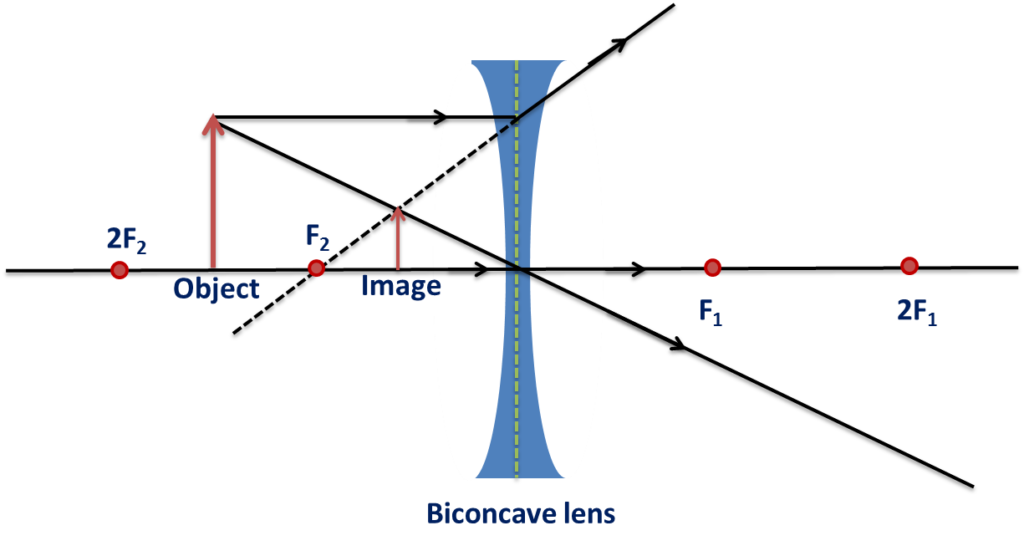
\includegraphics[width=.9\linewidth]{concave.png}
    \captionof{figure}{\centering Ray diagram of concave lens image formation \protect\cite{topprlensimage}.}
    \label{fig:concaveimage}
\end{minipage}
\hfill
\begin{minipage}{.45\textwidth}
    \captionsetup{hypcap=false}
    \centering
    
    \begin{table}[H]
        \centering
        \resizebox{.9\linewidth}{!}{

            \begin{tabular}{|c|c|c|c|}
            \hline
            \textbf{\begin{tabular}[c]{@{}c@{}}Object\\ Position\end{tabular}}     & \textbf{\begin{tabular}[c]{@{}c@{}}Image\\ Position\end{tabular}} & \textbf{\begin{tabular}[c]{@{}c@{}}Image\\ Size\end{tabular}}            & \textbf{\begin{tabular}[c]{@{}c@{}}Image\\ Nature\end{tabular}} \\ \hline
            \textbf{At infinity}                                                   & At $F_2$                                                          & \begin{tabular}[c]{@{}c@{}}Highly Diminished,\\ Point-Sized\end{tabular} & \begin{tabular}[c]{@{}c@{}}Virtual, \\ Upright\end{tabular}     \\ \hline
            \textbf{\begin{tabular}[c]{@{}c@{}}Object inside \\ lens\end{tabular}} & \begin{tabular}[c]{@{}c@{}}Between \\ lens and $F_2$\end{tabular} & Diminished                                                               & \begin{tabular}[c]{@{}c@{}}Virtual, \\ Upright\end{tabular}     \\ \hline
            \end{tabular}

        }
        \caption{\centering Table of the different cases of concave lens image formation \protect\cite{geekconcave,topprlensimage}}
        \label{tab:2}
    \end{table}
\end{minipage}

\subsection{Polarisation} \label{sec:1.2}

Since light, electromagnetic radiation, has both particle and (transverse) wave properties, it can be restricted to propagating in one direction, shown in figure \ref{fig:polar}
\cite{isaacpolar,britpolar}.
Light can be polarised by passing through certain materials, like crystals, that act as a filter 
\cite{britpolar}.

\begin{figure}[H]
    \centering
    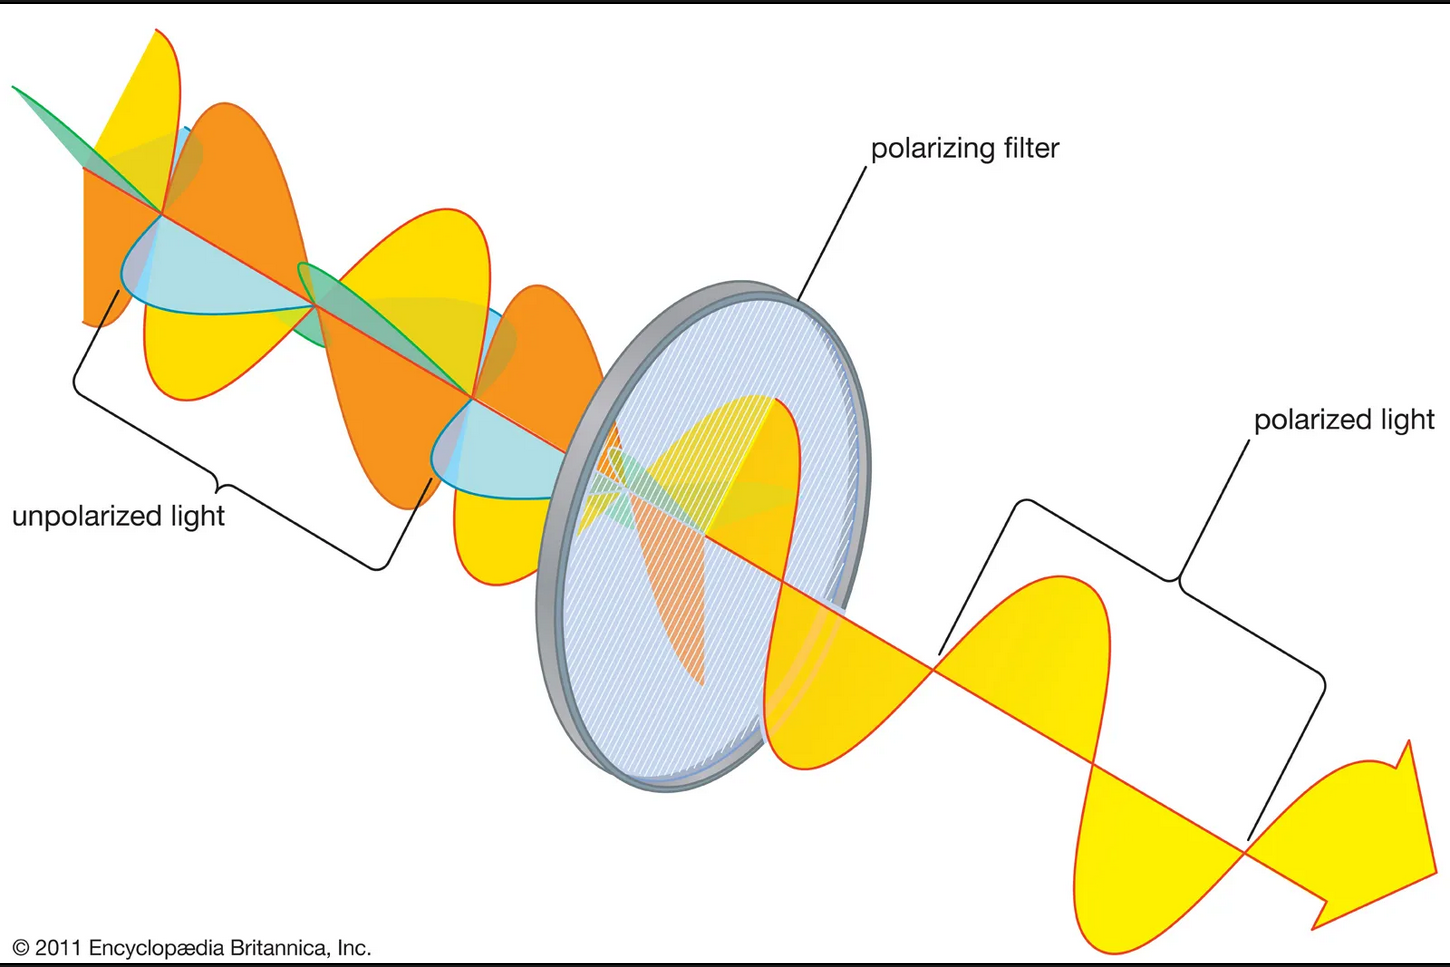
\includegraphics[width=10cm]{polarisation.png}
    \caption{\centering Visual representation of polarisation of light \protect\cite{britpolar}.}
    \label{fig:polar}
\end{figure}

\subsubsection{Reflection and Refraction} \label{sec:1.2.1}

\textbf{Reflection} is when the light rays change direction as they hit a surface, or travel through a medium that has a different chemical composition to the original medium
\cite{libreref,britref}.
For reflection to take place, the angle of incidence ($\theta_i$) must equal the angle of reflection ($\theta_r$), of which are measured with respect to the normal (perpendicular)
to the surface. This is known as the law of reflection
\cite{libreref,britref}.
Diffusion is a type of reflection on a rough surface, so the light rays reflect in many different directions
\cite{libreref}.

\textbf{Refraction} occurs when light travelling through a transparent medium encounters another transparent medium
\cite{britref}.
The variations in the matter of the medium causes the light to "bend" (change directions) as it is transmitted through the new medium
\cite{libreref}.
The law of refraction is more commonly known as \textit{Snell's Law}, §\ref{sec:1.2.2}.

\subsubsection{Snell's Law} \label{sec:1.2.2}

A ray of light changes directions when it passes from a medium of specificied refractive index (number indicating the magnitude of refraction of a medium)
through another medium of different refractive index
\cite{libreref}.

The below equation, equation \ref{eq:3}, is the mathematical description of Snell's Law, with $n_{1,2}$ as the refractive index of the two mediums, $\theta_i$ as the incident angle,
and $\theta_r$ as the refracive angle:

\begin{gather} \label{eq:3}
    n_1 \sin \theta_i = n_2 \sin \theta_r \quad \implies \quad \frac{n_2}{n_1} = \frac{\sin \theta_i}{\sin \theta_r}
\end{gather}

The angle at which the light is refracted is dependent on the refractive index of the medium, $\sin \theta \propto n$, so if the refracive index of the second medium is greater 
than the first medium the angle of refraction will be smaller
\cite{libresnell}.

\subsubsection{Brewster's Angle} \label{sec:1.2.3}

Light can be polarised by reflection and refraction, as seen in figure \ref{fig:brew}, where majority of the light will be reflected off the medium and the rest of the light
will be refracted through the medium. In doing so, the reflected ray gets partially polarised parallel to the medium's surface and the refracted ray get partially polarised perpendicular
to the surface of the medium
\cite{geekpolar}.

\begin{figure}[H]
    \centering
    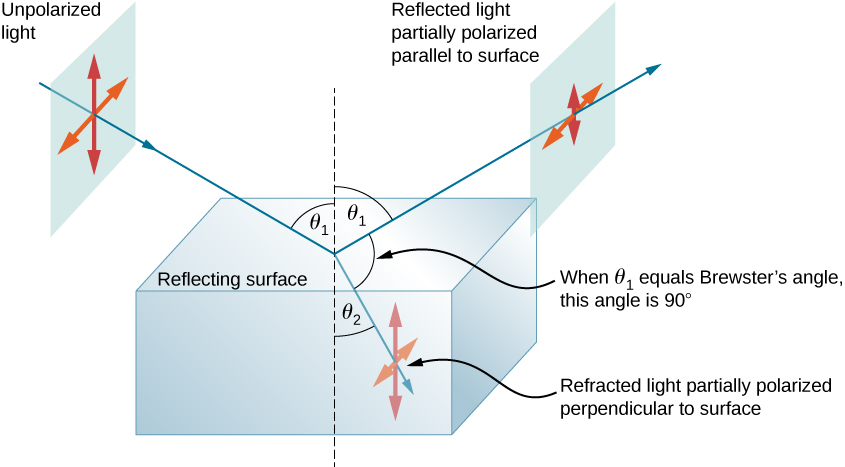
\includegraphics[width=12.5cm]{brewster.jpg}
    \caption{\centering Diagram of light polarisation with Brewster's angle \protect\cite{floridabrewster}.}
    \label{fig:brew}
\end{figure}

Brewster's angle is also known as the \textit{polarisation angle}, which is the incident angle at which unpolarised light is seperated into its vertical (perpendicular) and horizontal
(parallel) \break components when that light is transmitted through a medium such that the angle between the reflected and refracted ray is $90^{\circ}$, Brewster's angle ($\theta_B$)
\cite{scidirbrew, bostonbrew}.

Brewster's angle can be derived from Snell's law \cite{UCDlens,scidirbrew}:

\begin{gather} \label{eq:4}
    n_1 \sin \theta_i = n_2 \sin \theta_t \qquad \theta_i = \theta_B \: , \: \theta_i + \theta_t
\end{gather}
\begin{gather}\label{eq:5}
    \implies \quad n_1 \sin \theta_B = n_2 \sin (90^{\circ} - \theta_B) = n_2 \cos (\theta_B)
\end{gather}
\begin{gather} \label{eq:6}
    \implies \quad \frac{\sin \theta_B}{\cos \theta_B} = \tan \theta_B = \frac{n_2}{n_1} = n \qquad \therefore \: n = \tan \theta_B
\end{gather}

This equation (\ref{eq:6}) can be used to both calculate the polarisation angle ($\theta_B$) or the refractive index ($n$) of a material, depending on the values previously known.

\subsubsection{Ratios of Intensity} \label{sec:1.2.4}

By manipulation of Snell's law, equation \ref{eq:3}, ratios of the intensities of the reflected to the incident light of the polarised light can be found \cite{UCDlens}:

\begin{minipage}{.45\textwidth}
    \begin{gather} \label{eq:7}
        R_{parallel} = \frac{\tan^2 (\theta_i - \theta_t)}{\tan^2 (\theta_i + \theta_t)}
    \end{gather}
\end{minipage}
\hfill
\begin{minipage}{.45\textwidth}
    \begin{gather}
        R_{perpendicular} = \frac{\sin^2 (\theta_i - \theta_t)}{\sin^2 (\theta_i + \theta_t)}
    \end{gather}
\end{minipage}

\vspace{.5cm}

This is such that if $R=0$, light is fully transmitted through the medium (no reflection), and if $R=1$, all the light is reflected (no polarisation)
\cite{UCDlens}.

\section{Methodology} \label{sec:2}

\subsection{Determining the Focal Length} \label{sec:2.1}

\begin{figure}[H]
    \centering
    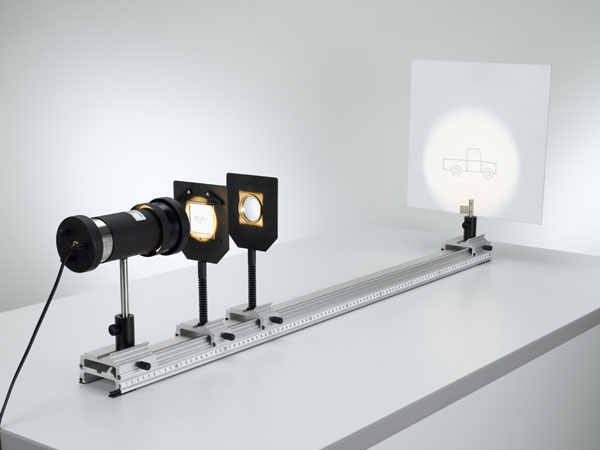
\includegraphics[width=10cm]{lens exp setup.jpg}
    \caption{\centering Experiment setup to determine the focal point of a convex lens \protect\cite{leyboldexp}.}
    \label{fig:lensexp}
\end{figure}

\subsubsection{Convex Lens Method} \label{sec:2.1.1}



\subsubsection{Concave Lens Method} \label{sec:2.1.2}



\subsection{Determining Brewster's Angle Method} \label{sec:2.2}

\begin{figure}[H]
    \centering
    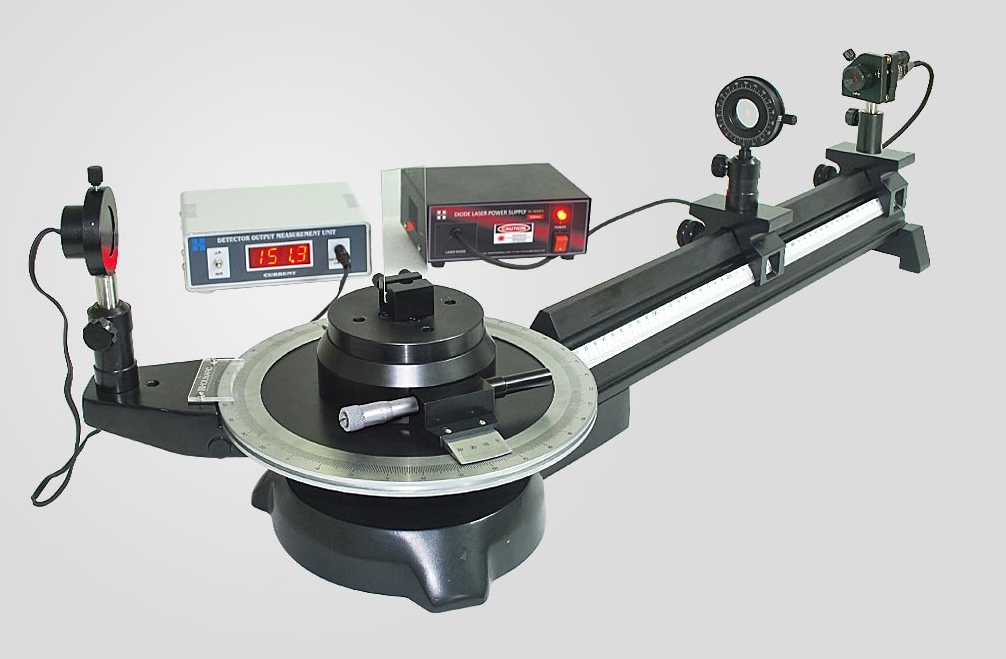
\includegraphics[width=10cm]{brewster exp.png}
    \caption{\centering Experiment setup to determing Brewster's angle \protect\cite{holmarcexp}.}
    \label{fig:brewexp}
\end{figure}

\section{Results and Calculations} \label{sec:3}

\subsection{Determining the Focal Length} \label{sec:3.1}

\subsubsection{Convex Lens} \label{sec:3.1.1}



\subsubsection{Concave Lense} \label{sec:3.1.2}



\subsection{Determining Brewster's Angle} \label{sec:3.2}



\section{Conclusion} \label{sec:4}


\section{Applications of Lenses}

\subsection{Eyeglasses}

\subsection{Microscopes}

\subsection{Telescopes}

\newpage

%%%%%%%%%%%%%%%%%%%%%%%%%%%%%%%%%%%

\bibliographystyle{IEEEtran}
\bibliography{References} \label{sec:ref}

\newpage

\section*{Appendix} \label{sec:A}
\addcontentsline{toc}{section}{Appendix}

\listoffigures

\listoftables

\subsection*{Raw Data}
\addcontentsline{toc}{subsection}{Raw Data}



\subsection*{Code}
\addcontentsline{toc}{subsection}{Code}



\end{document}